\documentclass[1p]{elsarticle_modified}
%\bibliographystyle{elsarticle-num}

%\usepackage[colorlinks]{hyperref}
%\usepackage{abbrmath_seonhwa} %\Abb, \Ascr, \Acal ,\Abf, \Afrak
\usepackage{amsfonts}
\usepackage{amssymb}
\usepackage{amsmath}
\usepackage{amsthm}
\usepackage{scalefnt}
\usepackage{amsbsy}
\usepackage{kotex}
\usepackage{caption}
\usepackage{subfig}
\usepackage{color}
\usepackage{graphicx}
\usepackage{xcolor} %% white, black, red, green, blue, cyan, magenta, yellow
\usepackage{float}
\usepackage{setspace}
\usepackage{hyperref}

\usepackage{tikz}
\usetikzlibrary{arrows}

\usepackage{multirow}
\usepackage{array} % fixed length table
\usepackage{hhline}

%%%%%%%%%%%%%%%%%%%%%
\makeatletter
\renewcommand*\env@matrix[1][\arraystretch]{%
	\edef\arraystretch{#1}%
	\hskip -\arraycolsep
	\let\@ifnextchar\new@ifnextchar
	\array{*\c@MaxMatrixCols c}}
\makeatother %https://tex.stackexchange.com/questions/14071/how-can-i-increase-the-line-spacing-in-a-matrix
%%%%%%%%%%%%%%%

\usepackage[normalem]{ulem}

\newcommand{\msout}[1]{\ifmmode\text{\sout{\ensuremath{#1}}}\else\sout{#1}\fi}
%SOURCE: \msout is \stkout macro in https://tex.stackexchange.com/questions/20609/strikeout-in-math-mode

\newcommand{\cancel}[1]{
	\ifmmode
	{\color{red}\msout{#1}}
	\else
	{\color{red}\sout{#1}}
	\fi
}

\newcommand{\add}[1]{
	{\color{blue}\uwave{#1}}
}

\newcommand{\replace}[2]{
	\ifmmode
	{\color{red}\msout{#1}}{\color{blue}\uwave{#2}}
	\else
	{\color{red}\sout{#1}}{\color{blue}\uwave{#2}}
	\fi
}

\newcommand{\Sol}{\mathcal{S}} %segment
\newcommand{\D}{D} %diagram
\newcommand{\A}{\mathcal{A}} %arc


%%%%%%%%%%%%%%%%%%%%%%%%%%%%%5 test

\def\sl{\operatorname{\textup{SL}}(2,\Cbb)}
\def\psl{\operatorname{\textup{PSL}}(2,\Cbb)}
\def\quan{\mkern 1mu \triangleright \mkern 1mu}

\theoremstyle{definition}
\newtheorem{thm}{Theorem}[section]
\newtheorem{prop}[thm]{Proposition}
\newtheorem{lem}[thm]{Lemma}
\newtheorem{ques}[thm]{Question}
\newtheorem{cor}[thm]{Corollary}
\newtheorem{defn}[thm]{Definition}
\newtheorem{exam}[thm]{Example}
\newtheorem{rmk}[thm]{Remark}
\newtheorem{alg}[thm]{Algorithm}

\newcommand{\I}{\sqrt{-1}}
\begin{document}

%\begin{frontmatter}
%
%\title{Boundary parabolic representations of knots up to 8 crossings}
%
%%% Group authors per affiliation:
%\author{Yunhi Cho} 
%\address{Department of Mathematics, University of Seoul, Seoul, Korea}
%\ead{yhcho@uos.ac.kr}
%
%
%\author{Seonhwa Kim} %\fnref{s_kim}}
%\address{Center for Geometry and Physics, Institute for Basic Science, Pohang, 37673, Korea}
%\ead{ryeona17@ibs.re.kr}
%
%\author{Hyuk Kim}
%\address{Department of Mathematical Sciences, Seoul National University, Seoul 08826, Korea}
%\ead{hyukkim@snu.ac.kr}
%
%\author{Seokbeom Yoon}
%\address{Department of Mathematical Sciences, Seoul National University, Seoul, 08826,  Korea}
%\ead{sbyoon15@snu.ac.kr}
%
%\begin{abstract}
%We find all boundary parabolic representation of knots up to 8 crossings.
%
%\end{abstract}
%\begin{keyword}
%    \MSC[2010] 57M25 
%\end{keyword}
%
%\end{frontmatter}

%\linenumbers
%\tableofcontents
%
\newcommand\colored[1]{\textcolor{white}{\rule[-0.35ex]{0.8em}{1.4ex}}\kern-0.8em\color{red} #1}%
%\newcommand\colored[1]{\textcolor{white}{ #1}\kern-2.17ex	\textcolor{white}{ #1}\kern-1.81ex	\textcolor{white}{ #1}\kern-2.15ex\color{red}#1	}

{\Large $\underline{12n_{0655}~(K12n_{0655})}$}

\setlength{\tabcolsep}{10pt}
\renewcommand{\arraystretch}{1.6}
\vspace{1cm}\begin{tabular}{m{100pt}>{\centering\arraybackslash}m{274pt}}
\multirow{5}{120pt}{
	\centering
	\includegraphics[width=112pt]{../../../GIT/diagram.site/Diagrams/png/2744_12n_0655.png}\\
\ \ \ A knot diagram\footnotemark}&
\allowdisplaybreaks
\textbf{Linearized knot diagam} \\
\cline{2-2}
 &
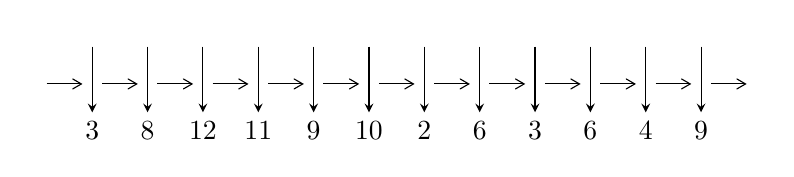
\begin{tikzpicture}[x=20pt, y=17pt]
	% nodes
	\node (C0) at (0, 0) {};
	\node (C1) at (1, 0) {};
	\node (C1U) at (1, +1) {};
	\node (C1D) at (1, -1) {3};

	\node (C2) at (2, 0) {};
	\node (C2U) at (2, +1) {};
	\node (C2D) at (2, -1) {8};

	\node (C3) at (3, 0) {};
	\node (C3U) at (3, +1) {};
	\node (C3D) at (3, -1) {12};

	\node (C4) at (4, 0) {};
	\node (C4U) at (4, +1) {};
	\node (C4D) at (4, -1) {11};

	\node (C5) at (5, 0) {};
	\node (C5U) at (5, +1) {};
	\node (C5D) at (5, -1) {9};

	\node (C6) at (6, 0) {};
	\node (C6U) at (6, +1) {};
	\node (C6D) at (6, -1) {10};

	\node (C7) at (7, 0) {};
	\node (C7U) at (7, +1) {};
	\node (C7D) at (7, -1) {2};

	\node (C8) at (8, 0) {};
	\node (C8U) at (8, +1) {};
	\node (C8D) at (8, -1) {6};

	\node (C9) at (9, 0) {};
	\node (C9U) at (9, +1) {};
	\node (C9D) at (9, -1) {3};

	\node (C10) at (10, 0) {};
	\node (C10U) at (10, +1) {};
	\node (C10D) at (10, -1) {6};

	\node (C11) at (11, 0) {};
	\node (C11U) at (11, +1) {};
	\node (C11D) at (11, -1) {4};

	\node (C12) at (12, 0) {};
	\node (C12U) at (12, +1) {};
	\node (C12D) at (12, -1) {9};
	\node (C13) at (13, 0) {};

	% arrows
	\draw[->,>={angle 60}]
	(C0) edge (C1) (C1) edge (C2) (C2) edge (C3) (C3) edge (C4) (C4) edge (C5) (C5) edge (C6) (C6) edge (C7) (C7) edge (C8) (C8) edge (C9) (C9) edge (C10) (C10) edge (C11) (C11) edge (C12) (C12) edge (C13) ;	\draw[->,>=stealth]
	(C1U) edge (C1D) (C2U) edge (C2D) (C3U) edge (C3D) (C4U) edge (C4D) (C5U) edge (C5D) (C6U) edge (C6D) (C7U) edge (C7D) (C8U) edge (C8D) (C9U) edge (C9D) (C10U) edge (C10D) (C11U) edge (C11D) (C12U) edge (C12D) ;
	\end{tikzpicture} \\
\hhline{~~} \\& 
\textbf{Solving Sequence} \\ \cline{2-2} 
 &
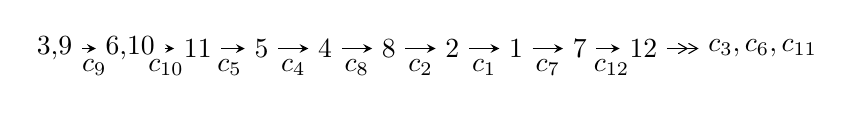
\begin{tikzpicture}[x=23pt, y=7pt]
	% node
	\node (A0) at (-1/8, 0) {3,9};
	\node (A1) at (17/16, 0) {6,10};
	\node (A2) at (17/8, 0) {11};
	\node (A3) at (25/8, 0) {5};
	\node (A4) at (33/8, 0) {4};
	\node (A5) at (41/8, 0) {8};
	\node (A6) at (49/8, 0) {2};
	\node (A7) at (57/8, 0) {1};
	\node (A8) at (65/8, 0) {7};
	\node (A9) at (73/8, 0) {12};
	\node (C1) at (1/2, -1) {$c_{9}$};
	\node (C2) at (13/8, -1) {$c_{10}$};
	\node (C3) at (21/8, -1) {$c_{5}$};
	\node (C4) at (29/8, -1) {$c_{4}$};
	\node (C5) at (37/8, -1) {$c_{8}$};
	\node (C6) at (45/8, -1) {$c_{2}$};
	\node (C7) at (53/8, -1) {$c_{1}$};
	\node (C8) at (61/8, -1) {$c_{7}$};
	\node (C9) at (69/8, -1) {$c_{12}$};
	\node (A10) at (11, 0) {$c_{3},c_{6},c_{11}$};

	% edge
	\draw[->,>=stealth]	
	(A0) edge (A1) (A1) edge (A2) (A2) edge (A3) (A3) edge (A4) (A4) edge (A5) (A5) edge (A6) (A6) edge (A7) (A7) edge (A8) (A8) edge (A9) ;
	\draw[->>,>={angle 60}]	
	(A9) edge (A10);
\end{tikzpicture} \\ 

\end{tabular} \\

\footnotetext{
The image of knot diagram is generated by the software ``\textbf{Draw programme}" developed by Andrew Bartholomew(\url{http://www.layer8.co.uk/maths/draw/index.htm\#Running-draw}), where we modified some parts for our purpose(\url{https://github.com/CATsTAILs/LinksPainter}).
}\phantom \\ \newline 
\centering \textbf{Ideals for irreducible components\footnotemark of $X_{\text{par}}$} 
 
\begin{align*}
I^u_{1}&=\langle 
8082770070 u^{10}+12874278132 u^9+\cdots+78579513703 b+583530199807,\\
\phantom{I^u_{1}}&\phantom{= \langle  }-10533832913358 u^{10}-20498499647469 u^9+\cdots+43925948159977 a-453136624250477,\\
\phantom{I^u_{1}}&\phantom{= \langle  }u^{11}+u^{10}-25 u^9+84 u^8-4 u^7-295 u^6+294 u^5+266 u^4-592 u^3+258 u^2+53 u-43\rangle \\
I^u_{2}&=\langle 
-13 u^{11}+11 u^{10}-7 u^9+26 u^8+50 u^7-47 u^6+8 u^5-54 u^4-44 u^3+10 u^2+46 b+21 u+53,\\
\phantom{I^u_{2}}&\phantom{= \langle  }8 u^{11}+18 u^{10}- u^9+30 u^8-52 u^7-33 u^6+11 u^5-57 u^4+66 u^3+54 u^2+23 a+26 u+1,\\
\phantom{I^u_{2}}&\phantom{= \langle  }u^{12}+2 u^{10}- u^9-2 u^8- u^7-3 u^6+2 u^5+2 u^4+4 u^3+u^2-1\rangle \\
I^u_{3}&=\langle 
b^2- b+1,\;a-1,\;u-1\rangle \\
\\
\end{align*}
\raggedright * 3 irreducible components of $\dim_{\mathbb{C}}=0$, with total 25 representations.\\
\footnotetext{All coefficients of polynomials are rational numbers. But the coefficients are sometimes approximated in decimal forms when there is not enough margin.}
\newpage
\renewcommand{\arraystretch}{1}
\centering \section*{I. $I^u_{1}= \langle 8.08\times10^{9} u^{10}+1.29\times10^{10} u^{9}+\cdots+7.86\times10^{10} b+5.84\times10^{11},\;-1.05\times10^{13} u^{10}-2.05\times10^{13} u^{9}+\cdots+4.39\times10^{13} a-4.53\times10^{14},\;u^{11}+u^{10}+\cdots+53 u-43 \rangle$}
\flushleft \textbf{(i) Arc colorings}\\
\begin{tabular}{m{7pt} m{180pt} m{7pt} m{180pt} }
\flushright $a_{3}=$&$\begin{pmatrix}0\\u\end{pmatrix}$ \\
\flushright $a_{9}=$&$\begin{pmatrix}1\\0\end{pmatrix}$ \\
\flushright $a_{6}=$&$\begin{pmatrix}0.239809 u^{10}+0.466660 u^{9}+\cdots-5.07748 u+10.3159\\-0.102861 u^{10}-0.163838 u^{9}+\cdots-2.44421 u-7.42598\end{pmatrix}$ \\
\flushright $a_{10}=$&$\begin{pmatrix}1\\u^2\end{pmatrix}$ \\
\flushright $a_{11}=$&$\begin{pmatrix}1.00685 u^{10}+1.73463 u^{9}+\cdots+5.81239 u+59.4569\\0.149991 u^{10}+0.294158 u^{9}+\cdots-2.04642 u+6.58542\end{pmatrix}$ \\
\flushright $a_{5}=$&$\begin{pmatrix}0.136948 u^{10}+0.302823 u^{9}+\cdots-7.52169 u+2.88994\\-0.102861 u^{10}-0.163838 u^{9}+\cdots-2.44421 u-7.42598\end{pmatrix}$ \\
\flushright $a_{4}=$&$\begin{pmatrix}-0.0526849 u^{10}-0.162132 u^{9}+\cdots+7.57873 u+2.62004\\0.214365 u^{10}+0.374779 u^{9}+\cdots+1.03850 u+11.9120\end{pmatrix}$ \\
\flushright $a_{8}=$&$\begin{pmatrix}-0.240845 u^{10}-0.364372 u^{9}+\cdots-6.91721 u-16.6179\\-0.192976 u^{10}-0.323582 u^{9}+\cdots-1.76300 u-11.8971\end{pmatrix}$ \\
\flushright $a_{2}=$&$\begin{pmatrix}0.672190 u^{10}+1.17359 u^{9}+\cdots+5.50874 u+38.9931\\0.241840 u^{10}+0.437101 u^{9}+\cdots+1.35348 u+12.9629\end{pmatrix}$ \\
\flushright $a_{1}=$&$\begin{pmatrix}0.672190 u^{10}+1.17359 u^{9}+\cdots+5.50874 u+38.9931\\-0.145871 u^{10}-0.264230 u^{9}+\cdots-0.976455 u-8.59734\end{pmatrix}$ \\
\flushright $a_{7}=$&$\begin{pmatrix}0.539583 u^{10}+0.987055 u^{9}+\cdots-4.34462 u+27.4965\\0.0516713 u^{10}+0.0842453 u^{9}+\cdots-1.24682 u+2.06071\end{pmatrix}$ \\
\flushright $a_{12}=$&$\begin{pmatrix}0.526320 u^{10}+0.909361 u^{9}+\cdots+4.53228 u+30.3957\\-0.145871 u^{10}-0.264230 u^{9}+\cdots-0.976455 u-8.59734\end{pmatrix}$\\&\end{tabular}
\flushleft \textbf{(ii) Obstruction class $= -1$}\\~\\
\flushleft \textbf{(iii) Cusp Shapes $= \frac{1137457766308}{1021533678139} u^{10}+\frac{2052116979712}{1021533678139} u^9+\cdots+\frac{13195254097138}{1021533678139} u+\frac{47127968197766}{1021533678139}$}\\~\\
\newpage\renewcommand{\arraystretch}{1}
\flushleft \textbf{(iv) u-Polynomials at the component}\newline \\
\begin{tabular}{m{50pt}|m{274pt}}
Crossings & \hspace{64pt}u-Polynomials at each crossing \\
\hline $$\begin{aligned}c_{1}\end{aligned}$$&$\begin{aligned}
&u^{11}+30 u^{10}+\cdots+46180 u+6241
\end{aligned}$\\
\hline $$\begin{aligned}c_{2},c_{7}\end{aligned}$$&$\begin{aligned}
&u^{11}+2 u^{10}+\cdots+290 u+79
\end{aligned}$\\
\hline $$\begin{aligned}c_{3},c_{4},c_{11}\end{aligned}$$&$\begin{aligned}
&u^{11}-3 u^{10}+\cdots-4 u+1
\end{aligned}$\\
\hline $$\begin{aligned}c_{5},c_{8}\end{aligned}$$&$\begin{aligned}
&u^{11}-6 u^{10}+\cdots+59 u+14
\end{aligned}$\\
\hline $$\begin{aligned}c_{6},c_{10}\end{aligned}$$&$\begin{aligned}
&u^{11}+16 u^{10}+\cdots-1205 u-239
\end{aligned}$\\
\hline $$\begin{aligned}c_{9}\end{aligned}$$&$\begin{aligned}
&u^{11}+u^{10}+\cdots+53 u-43
\end{aligned}$\\
\hline $$\begin{aligned}c_{12}\end{aligned}$$&$\begin{aligned}
&u^{11}+2 u^{10}+\cdots-9 u-4
\end{aligned}$\\
\hline
\end{tabular}\\~\\
\newpage\renewcommand{\arraystretch}{1}
\flushleft \textbf{(v) Riley Polynomials at the component}\newline \\
\begin{tabular}{m{50pt}|m{274pt}}
Crossings & \hspace{64pt}Riley Polynomials at each crossing \\
\hline $$\begin{aligned}c_{1}\end{aligned}$$&$\begin{aligned}
&y^{11}-270 y^{10}+\cdots+1320014200 y-38950081
\end{aligned}$\\
\hline $$\begin{aligned}c_{2},c_{7}\end{aligned}$$&$\begin{aligned}
&y^{11}-30 y^{10}+\cdots+46180 y-6241
\end{aligned}$\\
\hline $$\begin{aligned}c_{3},c_{4},c_{11}\end{aligned}$$&$\begin{aligned}
&y^{11}+9 y^{10}+\cdots+78 y-1
\end{aligned}$\\
\hline $$\begin{aligned}c_{5},c_{8}\end{aligned}$$&$\begin{aligned}
&y^{11}-24 y^{10}+\cdots+4069 y-196
\end{aligned}$\\
\hline $$\begin{aligned}c_{6},c_{10}\end{aligned}$$&$\begin{aligned}
&y^{11}-94 y^{10}+\cdots+639425 y-57121
\end{aligned}$\\
\hline $$\begin{aligned}c_{9}\end{aligned}$$&$\begin{aligned}
&y^{11}-51 y^{10}+\cdots+24997 y-1849
\end{aligned}$\\
\hline $$\begin{aligned}c_{12}\end{aligned}$$&$\begin{aligned}
&y^{11}-28 y^{10}+\cdots+289 y-16
\end{aligned}$\\
\hline
\end{tabular}\\~\\
\newpage\flushleft \textbf{(vi) Complex Volumes and Cusp Shapes}
$$\begin{array}{c|c|c}  
\text{Solutions to }I^u_{1}& \I (\text{vol} + \sqrt{-1}CS) & \text{Cusp shape}\\
 \hline 
\begin{aligned}
u &= \phantom{-}1.14783\phantom{ +0.000000I} \\
a &= -0.625800\phantom{ +0.000000I} \\
b &= \phantom{-}0.599073\phantom{ +0.000000I}\end{aligned}
 & -7.73425\phantom{ +0.000000I} & -2.27460\phantom{ +0.000000I} \\ \hline\begin{aligned}
u &= \phantom{-}0.961384 + 0.663629 I \\
a &= \phantom{-}0.896764 - 0.517452 I \\
b &= \phantom{-}0.196134 + 1.286040 I\end{aligned}
 & \phantom{-}1.65294 + 2.05058 I & -10.88896 - 3.66206 I \\ \hline\begin{aligned}
u &= \phantom{-}0.961384 - 0.663629 I \\
a &= \phantom{-}0.896764 + 0.517452 I \\
b &= \phantom{-}0.196134 - 1.286040 I\end{aligned}
 & \phantom{-}1.65294 - 2.05058 I & -10.88896 + 3.66206 I \\ \hline\begin{aligned}
u &= \phantom{-}0.729816 + 0.078717 I \\
a &= -2.86559 - 0.69887 I \\
b &= -0.674831 + 0.650678 I\end{aligned}
 & \phantom{-}9.56370 + 2.81490 I & -11.11373 - 3.91531 I \\ \hline\begin{aligned}
u &= \phantom{-}0.729816 - 0.078717 I \\
a &= -2.86559 + 0.69887 I \\
b &= -0.674831 - 0.650678 I\end{aligned}
 & \phantom{-}9.56370 - 2.81490 I & -11.11373 + 3.91531 I \\ \hline\begin{aligned}
u &= -1.47245 + 0.38796 I \\
a &= -0.199156 - 0.028059 I \\
b &= -1.09827 - 0.95568 I\end{aligned}
 & -1.22023 - 2.91334 I & -10.21854 + 2.00386 I \\ \hline\begin{aligned}
u &= -1.47245 - 0.38796 I \\
a &= -0.199156 + 0.028059 I \\
b &= -1.09827 + 0.95568 I\end{aligned}
 & -1.22023 + 2.91334 I & -10.21854 - 2.00386 I \\ \hline\begin{aligned}
u &= -0.357190\phantom{ +0.000000I} \\
a &= \phantom{-}0.642478\phantom{ +0.000000I} \\
b &= -0.230598\phantom{ +0.000000I}\end{aligned}
 & -0.556349\phantom{ +0.000000I} & -18.0810\phantom{ +0.000000I} \\ \hline\begin{aligned}
u &= \phantom{-}2.17516 + 2.14936 I \\
a &= \phantom{-}0.426144 - 0.535385 I \\
b &= \phantom{-}1.92336 + 1.67643 I\end{aligned}
 & -15.4000 - 9.3794 I & -9.97556 + 3.09821 I \\ \hline\begin{aligned}
u &= \phantom{-}2.17516 - 2.14936 I \\
a &= \phantom{-}0.426144 + 0.535385 I \\
b &= \phantom{-}1.92336 - 1.67643 I\end{aligned}
 & -15.4000 + 9.3794 I & -9.97556 - 3.09821 I\\
 \hline 
 \end{array}$$\newpage$$\begin{array}{c|c|c}  
\text{Solutions to }I^u_{1}& \I (\text{vol} + \sqrt{-1}CS) & \text{Cusp shape}\\
 \hline 
\begin{aligned}
u &= -6.57845\phantom{ +0.000000I} \\
a &= \phantom{-}0.327461\phantom{ +0.000000I} \\
b &= \phantom{-}4.93875\phantom{ +0.000000I}\end{aligned}
 & \phantom{-}17.4529\phantom{ +0.000000I} & -11.2510\phantom{ +0.000000I}\\
 \hline 
 \end{array}$$\newpage\newpage\renewcommand{\arraystretch}{1}
\centering \section*{II. $I^u_{2}= \langle -13 u^{11}+11 u^{10}+\cdots+46 b+53,\;8 u^{11}+18 u^{10}+\cdots+23 a+1,\;u^{12}+2 u^{10}+\cdots+u^2-1 \rangle$}
\flushleft \textbf{(i) Arc colorings}\\
\begin{tabular}{m{7pt} m{180pt} m{7pt} m{180pt} }
\flushright $a_{3}=$&$\begin{pmatrix}0\\u\end{pmatrix}$ \\
\flushright $a_{9}=$&$\begin{pmatrix}1\\0\end{pmatrix}$ \\
\flushright $a_{6}=$&$\begin{pmatrix}-0.347826 u^{11}-0.782609 u^{10}+\cdots-1.13043 u-0.0434783\\0.282609 u^{11}-0.239130 u^{10}+\cdots-0.456522 u-1.15217\end{pmatrix}$ \\
\flushright $a_{10}=$&$\begin{pmatrix}1\\u^2\end{pmatrix}$ \\
\flushright $a_{11}=$&$\begin{pmatrix}-1.02174 u^{11}+1.32609 u^{10}+\cdots+2.80435 u+0.934783\\u^2+1\end{pmatrix}$ \\
\flushright $a_{5}=$&$\begin{pmatrix}-0.0652174 u^{11}-1.02174 u^{10}+\cdots-1.58696 u-1.19565\\0.282609 u^{11}-0.239130 u^{10}+\cdots-0.456522 u-1.15217\end{pmatrix}$ \\
\flushright $a_{4}=$&$\begin{pmatrix}0.891304 u^{11}-0.369565 u^{10}+\cdots-1.97826 u-1.32609\\0.586957 u^{11}-0.804348 u^{10}+\cdots-0.717391 u-0.239130\end{pmatrix}$ \\
\flushright $a_{8}=$&$\begin{pmatrix}-0.456522 u^{11}-0.152174 u^{10}+\cdots-0.108696 u-0.369565\\0.282609 u^{11}-0.239130 u^{10}+\cdots-0.456522 u-1.15217\end{pmatrix}$ \\
\flushright $a_{2}=$&$\begin{pmatrix}0.630435 u^{11}-0.456522 u^{10}+\cdots-0.326087 u-0.108696\\0.239130 u^{11}+0.413043 u^{10}+\cdots+2.15217 u-0.282609\end{pmatrix}$ \\
\flushright $a_{1}=$&$\begin{pmatrix}0.630435 u^{11}-0.456522 u^{10}+\cdots-0.326087 u-0.108696\\0.391304 u^{11}+0.130435 u^{10}+\cdots+1.52174 u+0.173913\end{pmatrix}$ \\
\flushright $a_{7}=$&$\begin{pmatrix}0.108696 u^{11}-0.630435 u^{10}+\cdots-1.02174 u+0.326087\\-1\end{pmatrix}$ \\
\flushright $a_{12}=$&$\begin{pmatrix}1.02174 u^{11}-0.326087 u^{10}+\cdots+1.19565 u+0.0652174\\0.391304 u^{11}+0.130435 u^{10}+\cdots+1.52174 u+0.173913\end{pmatrix}$\\&\end{tabular}
\flushleft \textbf{(ii) Obstruction class $= 1$}\\~\\
\flushleft \textbf{(iii) Cusp Shapes $= \frac{18}{23} u^{11}-\frac{63}{23} u^{10}+\frac{84}{23} u^9-\frac{151}{23} u^8+\frac{113}{23} u^7+\frac{58}{23} u^6-\frac{50}{23} u^5+\frac{188}{23} u^4-\frac{139}{23} u^3-\frac{74}{23} u^2-\frac{160}{23} u-\frac{153}{23}$}\\~\\
\newpage\renewcommand{\arraystretch}{1}
\flushleft \textbf{(iv) u-Polynomials at the component}\newline \\
\begin{tabular}{m{50pt}|m{274pt}}
Crossings & \hspace{64pt}u-Polynomials at each crossing \\
\hline $$\begin{aligned}c_{1}\end{aligned}$$&$\begin{aligned}
&u^{12}-12 u^{11}+\cdots-14 u+1
\end{aligned}$\\
\hline $$\begin{aligned}c_{2}\end{aligned}$$&$\begin{aligned}
&u^{12}-6 u^{10}+u^9+15 u^8-4 u^7-21 u^6+5 u^5+17 u^4-3 u^3-7 u^2+1
\end{aligned}$\\
\hline $$\begin{aligned}c_{3},c_{4}\end{aligned}$$&$\begin{aligned}
&u^{12}+u^{11}+\cdots-2 u^2-1
\end{aligned}$\\
\hline $$\begin{aligned}c_{5}\end{aligned}$$&$\begin{aligned}
&u^{12}-3 u^{11}+5 u^{10}-5 u^9+5 u^7-5 u^6+2 u^5+3 u^4-3 u^3-1
\end{aligned}$\\
\hline $$\begin{aligned}c_{6}\end{aligned}$$&$\begin{aligned}
&u^{12}+3 u^9-3 u^8-2 u^7+5 u^6-5 u^5+5 u^3-5 u^2+3 u-1
\end{aligned}$\\
\hline $$\begin{aligned}c_{7}\end{aligned}$$&$\begin{aligned}
&u^{12}-6 u^{10}- u^9+15 u^8+4 u^7-21 u^6-5 u^5+17 u^4+3 u^3-7 u^2+1
\end{aligned}$\\
\hline $$\begin{aligned}c_{8}\end{aligned}$$&$\begin{aligned}
&u^{12}+3 u^{11}+5 u^{10}+5 u^9-5 u^7-5 u^6-2 u^5+3 u^4+3 u^3-1
\end{aligned}$\\
\hline $$\begin{aligned}c_{9}\end{aligned}$$&$\begin{aligned}
&u^{12}+2 u^{10}- u^9-2 u^8- u^7-3 u^6+2 u^5+2 u^4+4 u^3+u^2-1
\end{aligned}$\\
\hline $$\begin{aligned}c_{10}\end{aligned}$$&$\begin{aligned}
&u^{12}-3 u^9-3 u^8+2 u^7+5 u^6+5 u^5-5 u^3-5 u^2-3 u-1
\end{aligned}$\\
\hline $$\begin{aligned}c_{11}\end{aligned}$$&$\begin{aligned}
&u^{12}- u^{11}+\cdots-2 u^2-1
\end{aligned}$\\
\hline $$\begin{aligned}c_{12}\end{aligned}$$&$\begin{aligned}
&u^{12}-4 u^{11}+\cdots+14 u+13
\end{aligned}$\\
\hline
\end{tabular}\\~\\
\newpage\renewcommand{\arraystretch}{1}
\flushleft \textbf{(v) Riley Polynomials at the component}\newline \\
\begin{tabular}{m{50pt}|m{274pt}}
Crossings & \hspace{64pt}Riley Polynomials at each crossing \\
\hline $$\begin{aligned}c_{1}\end{aligned}$$&$\begin{aligned}
&y^{12}-12 y^{11}+\cdots-30 y+1
\end{aligned}$\\
\hline $$\begin{aligned}c_{2},c_{7}\end{aligned}$$&$\begin{aligned}
&y^{12}-12 y^{11}+\cdots-14 y+1
\end{aligned}$\\
\hline $$\begin{aligned}c_{3},c_{4},c_{11}\end{aligned}$$&$\begin{aligned}
&y^{12}+15 y^{11}+\cdots+4 y+1
\end{aligned}$\\
\hline $$\begin{aligned}c_{5},c_{8}\end{aligned}$$&$\begin{aligned}
&y^{12}+y^{11}+\cdots-6 y^2+1
\end{aligned}$\\
\hline $$\begin{aligned}c_{6},c_{10}\end{aligned}$$&$\begin{aligned}
&y^{12}-6 y^{10}+\cdots+y+1
\end{aligned}$\\
\hline $$\begin{aligned}c_{9}\end{aligned}$$&$\begin{aligned}
&y^{12}+4 y^{11}+\cdots-2 y+1
\end{aligned}$\\
\hline $$\begin{aligned}c_{12}\end{aligned}$$&$\begin{aligned}
&y^{12}-18 y^{11}+\cdots+298 y+169
\end{aligned}$\\
\hline
\end{tabular}\\~\\
\newpage\flushleft \textbf{(vi) Complex Volumes and Cusp Shapes}
$$\begin{array}{c|c|c}  
\text{Solutions to }I^u_{2}& \I (\text{vol} + \sqrt{-1}CS) & \text{Cusp shape}\\
 \hline 
\begin{aligned}
u &= -0.290321 + 0.812321 I \\
a &= \phantom{-}1.60962 + 2.31665 I \\
b &= -0.148186 - 0.670337 I\end{aligned}
 & \phantom{-}10.30340 - 2.52674 I & -1.40798 + 1.03113 I \\ \hline\begin{aligned}
u &= -0.290321 - 0.812321 I \\
a &= \phantom{-}1.60962 - 2.31665 I \\
b &= -0.148186 + 0.670337 I\end{aligned}
 & \phantom{-}10.30340 + 2.52674 I & -1.40798 - 1.03113 I \\ \hline\begin{aligned}
u &= -1.14608\phantom{ +0.000000I} \\
a &= -0.443256\phantom{ +0.000000I} \\
b &= \phantom{-}0.750402\phantom{ +0.000000I}\end{aligned}
 & -8.04457\phantom{ +0.000000I} & -28.6700\phantom{ +0.000000I} \\ \hline\begin{aligned}
u &= \phantom{-}1.126080 + 0.271306 I \\
a &= -0.106545 + 0.615518 I \\
b &= \phantom{-}0.727354 + 0.248918 I\end{aligned}
 & -3.20078 - 2.30167 I & -14.2286 + 2.6049 I \\ \hline\begin{aligned}
u &= \phantom{-}1.126080 - 0.271306 I \\
a &= -0.106545 - 0.615518 I \\
b &= \phantom{-}0.727354 - 0.248918 I\end{aligned}
 & -3.20078 + 2.30167 I & -14.2286 - 2.6049 I \\ \hline\begin{aligned}
u &= \phantom{-}0.184248 + 1.148890 I \\
a &= \phantom{-}0.47497 - 1.34357 I \\
b &= -0.296082 + 1.038070 I\end{aligned}
 & \phantom{-}2.61823 + 1.74326 I & -3.69799 - 2.86039 I \\ \hline\begin{aligned}
u &= \phantom{-}0.184248 - 1.148890 I \\
a &= \phantom{-}0.47497 + 1.34357 I \\
b &= -0.296082 - 1.038070 I\end{aligned}
 & \phantom{-}2.61823 - 1.74326 I & -3.69799 + 2.86039 I \\ \hline\begin{aligned}
u &= -0.564251 + 0.474715 I \\
a &= -1.270550 - 0.606648 I \\
b &= -1.199700 + 0.382821 I\end{aligned}
 & \phantom{-}0.75595 + 3.94751 I & -8.05344 - 4.79157 I \\ \hline\begin{aligned}
u &= -0.564251 - 0.474715 I \\
a &= -1.270550 + 0.606648 I \\
b &= -1.199700 - 0.382821 I\end{aligned}
 & \phantom{-}0.75595 - 3.94751 I & -8.05344 + 4.79157 I \\ \hline\begin{aligned}
u &= \phantom{-}0.524737\phantom{ +0.000000I} \\
a &= -1.48305\phantom{ +0.000000I} \\
b &= -1.22481\phantom{ +0.000000I}\end{aligned}
 & -3.37867\phantom{ +0.000000I} & -11.4520\phantom{ +0.000000I}\\
 \hline 
 \end{array}$$\newpage$$\begin{array}{c|c|c}  
\text{Solutions to }I^u_{2}& \I (\text{vol} + \sqrt{-1}CS) & \text{Cusp shape}\\
 \hline 
\begin{aligned}
u &= -0.14508 + 1.49712 I \\
a &= \phantom{-}0.255664 + 0.886834 I \\
b &= -0.34618 - 1.41208 I\end{aligned}
 & \phantom{-}5.10447 - 1.33905 I & -8.55072 + 1.28965 I \\ \hline\begin{aligned}
u &= -0.14508 - 1.49712 I \\
a &= \phantom{-}0.255664 - 0.886834 I \\
b &= -0.34618 + 1.41208 I\end{aligned}
 & \phantom{-}5.10447 + 1.33905 I & -8.55072 - 1.28965 I\\
 \hline 
 \end{array}$$\newpage\newpage\renewcommand{\arraystretch}{1}
\centering \section*{III. $I^u_{3}= \langle b^2- b+1,\;a-1,\;u-1 \rangle$}
\flushleft \textbf{(i) Arc colorings}\\
\begin{tabular}{m{7pt} m{180pt} m{7pt} m{180pt} }
\flushright $a_{3}=$&$\begin{pmatrix}0\\1\end{pmatrix}$ \\
\flushright $a_{9}=$&$\begin{pmatrix}1\\0\end{pmatrix}$ \\
\flushright $a_{6}=$&$\begin{pmatrix}1\\b\end{pmatrix}$ \\
\flushright $a_{10}=$&$\begin{pmatrix}1\\1\end{pmatrix}$ \\
\flushright $a_{11}=$&$\begin{pmatrix}b\\0\end{pmatrix}$ \\
\flushright $a_{5}=$&$\begin{pmatrix}b+1\\b\end{pmatrix}$ \\
\flushright $a_{4}=$&$\begin{pmatrix}b\\b\end{pmatrix}$ \\
\flushright $a_{8}=$&$\begin{pmatrix}- b+1\\- b+1\end{pmatrix}$ \\
\flushright $a_{2}=$&$\begin{pmatrix}- b\\- b+1\end{pmatrix}$ \\
\flushright $a_{1}=$&$\begin{pmatrix}- b\\1\end{pmatrix}$ \\
\flushright $a_{7}=$&$\begin{pmatrix}- b+2\\1\end{pmatrix}$ \\
\flushright $a_{12}=$&$\begin{pmatrix}- b+1\\1\end{pmatrix}$\\&\end{tabular}
\flushleft \textbf{(ii) Obstruction class $= -1$}\\~\\
\flushleft \textbf{(iii) Cusp Shapes $= -4 b-7$}\\~\\
\newpage\renewcommand{\arraystretch}{1}
\flushleft \textbf{(iv) u-Polynomials at the component}\newline \\
\begin{tabular}{m{50pt}|m{274pt}}
Crossings & \hspace{64pt}u-Polynomials at each crossing \\
\hline $$\begin{aligned}c_{1},c_{2},c_{5}\\c_{7},c_{8}\end{aligned}$$&$\begin{aligned}
&u^2- u+1
\end{aligned}$\\
\hline $$\begin{aligned}c_{3},c_{4},c_{6}\\c_{10},c_{11}\end{aligned}$$&$\begin{aligned}
&u^2+u+1
\end{aligned}$\\
\hline $$\begin{aligned}c_{9},c_{12}\end{aligned}$$&$\begin{aligned}
&(u-1)^2
\end{aligned}$\\
\hline
\end{tabular}\\~\\
\newpage\renewcommand{\arraystretch}{1}
\flushleft \textbf{(v) Riley Polynomials at the component}\newline \\
\begin{tabular}{m{50pt}|m{274pt}}
Crossings & \hspace{64pt}Riley Polynomials at each crossing \\
\hline $$\begin{aligned}c_{1},c_{2},c_{3}\\c_{4},c_{5},c_{6}\\c_{7},c_{8},c_{10}\\c_{11}\end{aligned}$$&$\begin{aligned}
&y^2+y+1
\end{aligned}$\\
\hline $$\begin{aligned}c_{9},c_{12}\end{aligned}$$&$\begin{aligned}
&(y-1)^2
\end{aligned}$\\
\hline
\end{tabular}\\~\\
\newpage\flushleft \textbf{(vi) Complex Volumes and Cusp Shapes}
$$\begin{array}{c|c|c}  
\text{Solutions to }I^u_{3}& \I (\text{vol} + \sqrt{-1}CS) & \text{Cusp shape}\\
 \hline 
\begin{aligned}
u &= \phantom{-}1.00000\phantom{ +0.000000I} \\
a &= \phantom{-}1.00000\phantom{ +0.000000I} \\
b &= \phantom{-}0.500000 + 0.866025 I\end{aligned}
 & \phantom{-}1.64493 + 2.02988 I & -9.00000 - 3.46410 I \\ \hline\begin{aligned}
u &= \phantom{-}1.00000\phantom{ +0.000000I} \\
a &= \phantom{-}1.00000\phantom{ +0.000000I} \\
b &= \phantom{-}0.500000 - 0.866025 I\end{aligned}
 & \phantom{-}1.64493 - 2.02988 I & -9.00000 + 3.46410 I\\
 \hline 
 \end{array}$$\newpage
\newpage\renewcommand{\arraystretch}{1}
\centering \section*{ IV. u-Polynomials}
\begin{tabular}{m{50pt}|m{274pt}}
Crossings & \hspace{64pt}u-Polynomials at each crossing \\
\hline $$\begin{aligned}c_{1}\end{aligned}$$&$\begin{aligned}
&(u^2- u+1)(u^{11}+30 u^{10}+\cdots+46180 u+6241)\\
&\cdot(u^{12}-12 u^{11}+\cdots-14 u+1)
\end{aligned}$\\
\hline $$\begin{aligned}c_{2}\end{aligned}$$&$\begin{aligned}
&(u^2- u+1)(u^{11}+2 u^{10}+\cdots+290 u+79)\\
&\cdot(u^{12}-6 u^{10}+u^9+15 u^8-4 u^7-21 u^6+5 u^5+17 u^4-3 u^3-7 u^2+1)
\end{aligned}$\\
\hline $$\begin{aligned}c_{3},c_{4}\end{aligned}$$&$\begin{aligned}
&(u^2+u+1)(u^{11}-3 u^{10}+\cdots-4 u+1)(u^{12}+u^{11}+\cdots-2 u^2-1)
\end{aligned}$\\
\hline $$\begin{aligned}c_{5}\end{aligned}$$&$\begin{aligned}
&(u^2- u+1)(u^{11}-6 u^{10}+\cdots+59 u+14)\\
&\cdot(u^{12}-3 u^{11}+5 u^{10}-5 u^9+5 u^7-5 u^6+2 u^5+3 u^4-3 u^3-1)
\end{aligned}$\\
\hline $$\begin{aligned}c_{6}\end{aligned}$$&$\begin{aligned}
&(u^2+u+1)(u^{11}+16 u^{10}+\cdots-1205 u-239)\\
&\cdot(u^{12}+3 u^9-3 u^8-2 u^7+5 u^6-5 u^5+5 u^3-5 u^2+3 u-1)
\end{aligned}$\\
\hline $$\begin{aligned}c_{7}\end{aligned}$$&$\begin{aligned}
&(u^2- u+1)(u^{11}+2 u^{10}+\cdots+290 u+79)\\
&\cdot(u^{12}-6 u^{10}- u^9+15 u^8+4 u^7-21 u^6-5 u^5+17 u^4+3 u^3-7 u^2+1)
\end{aligned}$\\
\hline $$\begin{aligned}c_{8}\end{aligned}$$&$\begin{aligned}
&(u^2- u+1)(u^{11}-6 u^{10}+\cdots+59 u+14)\\
&\cdot(u^{12}+3 u^{11}+5 u^{10}+5 u^9-5 u^7-5 u^6-2 u^5+3 u^4+3 u^3-1)
\end{aligned}$\\
\hline $$\begin{aligned}c_{9}\end{aligned}$$&$\begin{aligned}
&((u-1)^2)(u^{11}+u^{10}+\cdots+53 u-43)\\
&\cdot(u^{12}+2 u^{10}- u^9-2 u^8- u^7-3 u^6+2 u^5+2 u^4+4 u^3+u^2-1)
\end{aligned}$\\
\hline $$\begin{aligned}c_{10}\end{aligned}$$&$\begin{aligned}
&(u^2+u+1)(u^{11}+16 u^{10}+\cdots-1205 u-239)\\
&\cdot(u^{12}-3 u^9-3 u^8+2 u^7+5 u^6+5 u^5-5 u^3-5 u^2-3 u-1)
\end{aligned}$\\
\hline $$\begin{aligned}c_{11}\end{aligned}$$&$\begin{aligned}
&(u^2+u+1)(u^{11}-3 u^{10}+\cdots-4 u+1)(u^{12}- u^{11}+\cdots-2 u^2-1)
\end{aligned}$\\
\hline $$\begin{aligned}c_{12}\end{aligned}$$&$\begin{aligned}
&((u-1)^2)(u^{11}+2 u^{10}+\cdots-9 u-4)(u^{12}-4 u^{11}+\cdots+14 u+13)
\end{aligned}$\\
\hline
\end{tabular}\newpage\renewcommand{\arraystretch}{1}
\centering \section*{ V. Riley Polynomials}
\begin{tabular}{m{50pt}|m{274pt}}
Crossings & \hspace{64pt}Riley Polynomials at each crossing \\
\hline $$\begin{aligned}c_{1}\end{aligned}$$&$\begin{aligned}
&(y^2+y+1)(y^{11}-270 y^{10}+\cdots+1.32001\times10^{9} y-3.89501\times10^{7})\\
&\cdot(y^{12}-12 y^{11}+\cdots-30 y+1)
\end{aligned}$\\
\hline $$\begin{aligned}c_{2},c_{7}\end{aligned}$$&$\begin{aligned}
&(y^2+y+1)(y^{11}-30 y^{10}+\cdots+46180 y-6241)\\
&\cdot(y^{12}-12 y^{11}+\cdots-14 y+1)
\end{aligned}$\\
\hline $$\begin{aligned}c_{3},c_{4},c_{11}\end{aligned}$$&$\begin{aligned}
&(y^2+y+1)(y^{11}+9 y^{10}+\cdots+78 y-1)(y^{12}+15 y^{11}+\cdots+4 y+1)
\end{aligned}$\\
\hline $$\begin{aligned}c_{5},c_{8}\end{aligned}$$&$\begin{aligned}
&(y^2+y+1)(y^{11}-24 y^{10}+\cdots+4069 y-196)(y^{12}+y^{11}+\cdots-6 y^2+1)
\end{aligned}$\\
\hline $$\begin{aligned}c_{6},c_{10}\end{aligned}$$&$\begin{aligned}
&(y^2+y+1)(y^{11}-94 y^{10}+\cdots+639425 y-57121)\\
&\cdot(y^{12}-6 y^{10}+\cdots+y+1)
\end{aligned}$\\
\hline $$\begin{aligned}c_{9}\end{aligned}$$&$\begin{aligned}
&((y-1)^2)(y^{11}-51 y^{10}+\cdots+24997 y-1849)\\
&\cdot(y^{12}+4 y^{11}+\cdots-2 y+1)
\end{aligned}$\\
\hline $$\begin{aligned}c_{12}\end{aligned}$$&$\begin{aligned}
&((y-1)^2)(y^{11}-28 y^{10}+\cdots+289 y-16)\\
&\cdot(y^{12}-18 y^{11}+\cdots+298 y+169)
\end{aligned}$\\
\hline
\end{tabular}
\vskip 2pc
\end{document}